% Generated by scripts/paper_tables.py from r7b-calibration/ -- do not edit by hand.
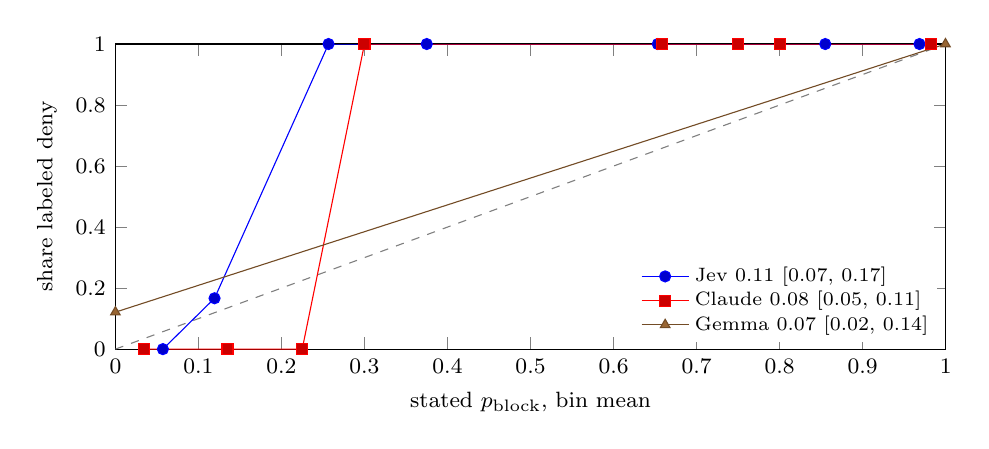
\begin{tikzpicture}
\begin{axis}[width=\columnwidth, height=0.45\columnwidth, xmin=0, xmax=1, ymin=0, ymax=1,
  xlabel={stated $p_\mathrm{block}$, bin mean}, ylabel={share labeled deny},
  legend cell align=left,
  legend style={font=\scriptsize, draw=none, inner sep=1pt, row sep=-2pt, at={(0.99,0.02)},
    anchor=south east},
  tick label style={font=\footnotesize}, label style={font=\footnotesize}]
\addplot[gray, dashed, domain=0:1, forget plot] {x};
\addplot+[mark=*] coordinates {(0.0572,0.0000) (0.1194,0.1667) (0.2567,1.0000) (0.3750,1.0000) (0.6533,1.0000) (0.8550,1.0000) (0.9685,1.0000)};
\addlegendentry{Jev 0.11 [0.07, 0.17]}
\addplot+[mark=square*] coordinates {(0.0343,0.0000) (0.1350,0.0000) (0.2250,0.0000) (0.3000,1.0000) (0.6583,1.0000) (0.7500,1.0000) (0.8000,1.0000) (0.9827,1.0000)};
\addlegendentry{Claude 0.08 [0.05, 0.11]}
\addplot+[mark=triangle*] coordinates {(0.0000,0.1212) (0.9998,1.0000)};
\addlegendentry{Gemma 0.07 [0.02, 0.14]}
\end{axis}
\end{tikzpicture}
